\documentclass{article}
\usepackage{pgf-umlcd}
%xeCJK
\usepackage[BoldFont,SlantFont,CJKchecksingle]{xeCJK}
\setCJKmainfont[BoldFont=SimHei,SlantedFont=KaiTi]{SimSun}

\begin{document}
\section{App Layer}
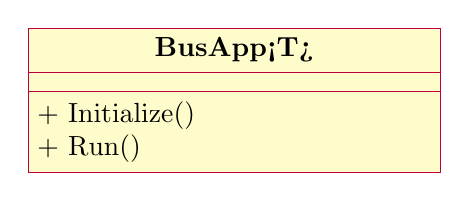
\begin{tikzpicture}
\begin{class}{BusApp<T>}{0,0}
\operation{+ Initialize()}
\operation{+ Run()}
\end{class}
\end{tikzpicture}
\newpage

\section{Window Layer}
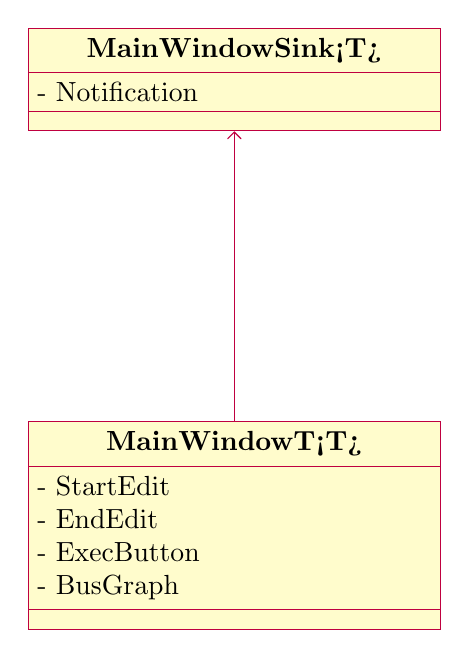
\begin{tikzpicture}
\begin{class}{MainWindowSink<T>}{0,0}
\attribute{- Notification}
\end{class}
\begin{class}{MainWindowT<T>}{0,-5}
\attribute{- StartEdit}
\attribute{- EndEdit}
\attribute{- ExecButton}
\attribute{- BusGraph}
\end{class}
\unidirectionalAssociation{MainWindowT<T>}{}{}{MainWindowSink<T>}
\end{tikzpicture}
\newpage

\section{View Layer}
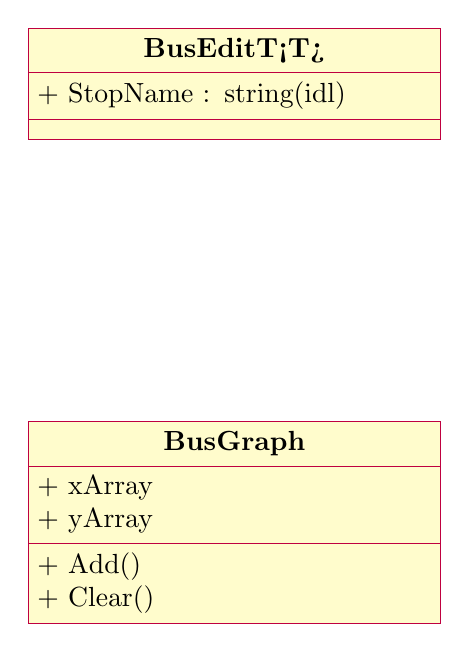
\begin{tikzpicture}
\begin{class}{BusEditT<T>}{0,0}
\attribute{+ StopName : string(idl)}
\end{class}
\begin{class}{BusGraph}{0,-5}
\attribute{+ xArray}
\attribute{+ yArray}
\operation{+ Add()}
\operation{+ Clear()}
\end{class}
\end{tikzpicture}
\newpage

\section{ViewModel Layer}
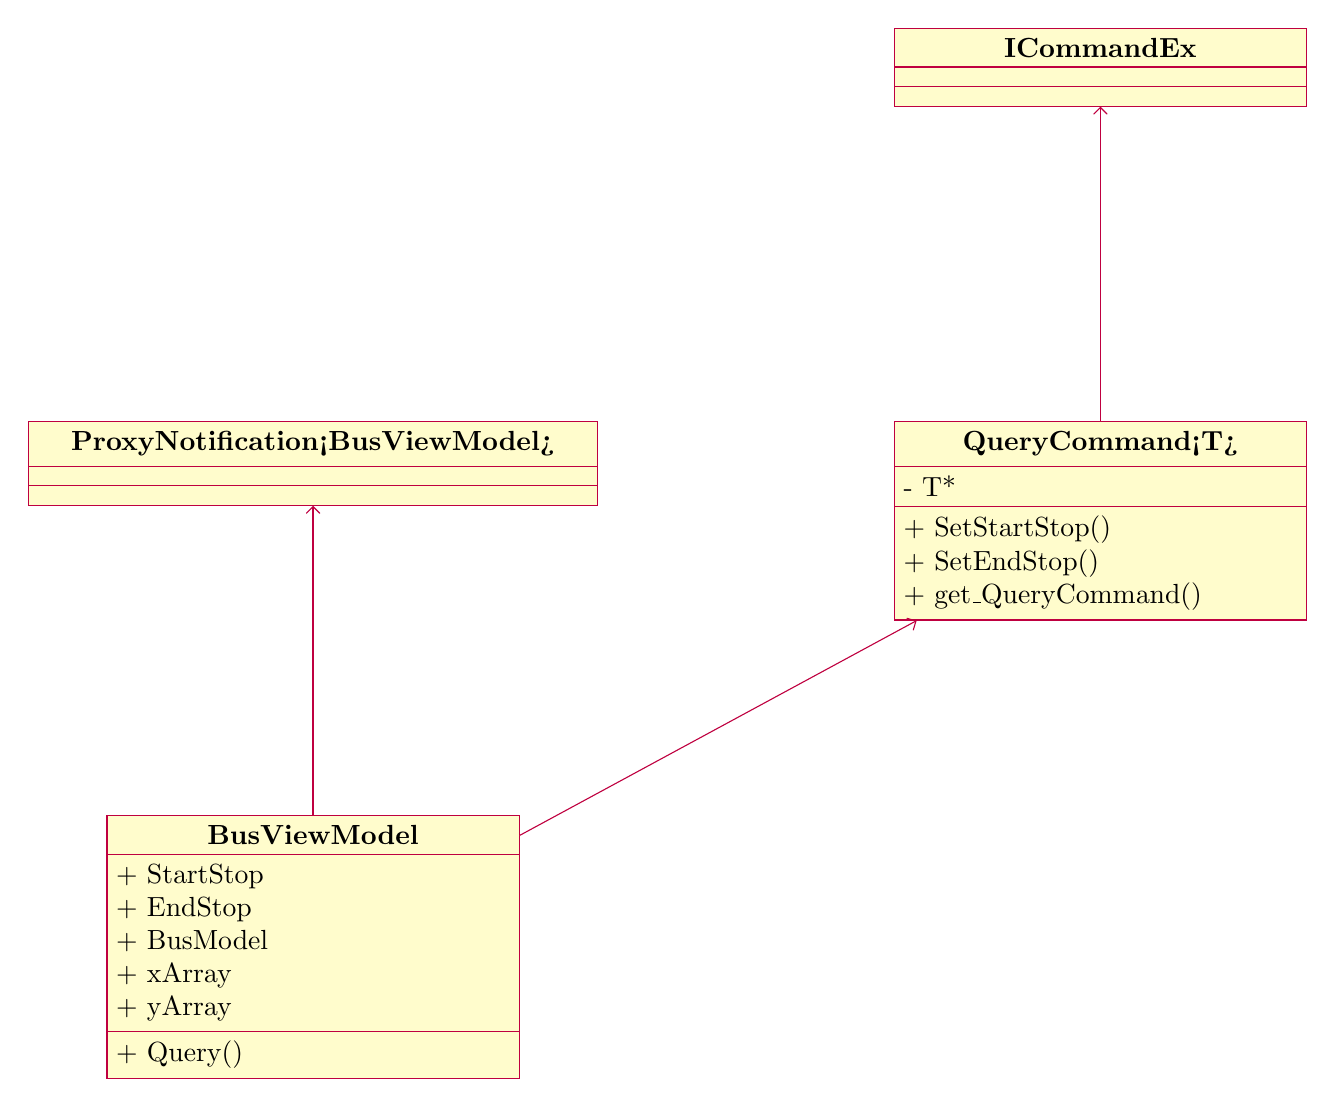
\begin{tikzpicture}
\begin{class}{ICommandEx}{10,5}\end{class}
\begin{class}{QueryCommand<T>}{10,0}
\attribute{- T*}
\operation{+ SetStartStop()}
\operation{+ SetEndStop()}
\operation{+ get\_QueryCommand()}
\end{class}
\begin{class}[text width=7cm]{ProxyNotification<BusViewModel>}{0,0}\end{class}
\begin{class}{BusViewModel}{0,-5}
\attribute{+ StartStop}
\attribute{+ EndStop}
\attribute{+ BusModel}
\attribute{+ xArray}
\attribute{+ yArray}
\operation{+ Query()}
\end{class}
\unidirectionalAssociation{QueryCommand<T>}{}{}{ICommandEx}
\unidirectionalAssociation{BusViewModel}{}{}{ProxyNotification<BusViewModel>}
\unidirectionalAssociation{BusViewModel}{}{}{QueryCommand<T>}
\end{tikzpicture}
\newpage

\section{Model Layer}
\begin{tikzpicture}
\begin{class}{Station}{0,0}
\attribute{+ name : string(idl)}
\attribute{+ x : double}
\attribute{+ y : double}
\operation{+ SetParameters()}
\end{class}
\begin{class}{BusRoute}{0,-5}
\attribute{+ Number: int}
\attribute{+ BusStop : Station}
\operation{+ Clear()}
\operation{+ Add()}
\end{class}
\begin{class}{RouteSet}{0,-10}
\attribute{+ Number: int}
\attribute{+ BusLine : BusRoute}
\operation{+ Add()}
\operation{+ Clear()}
\end{class}
\begin{class}{BusDataModel}{0,-15}
\attribute{+ RouteSet : RouteSet}
\operation{+ Query()}
\end{class}
\begin{class}{BusStorageHelper}{10,-15}
\operation{+ Load()}
\operation{+ Save()}
\end{class}
\unidirectionalAssociation{BusRoute}{* -端2}{1 -端1}{Station}
\unidirectionalAssociation{RouteSet}{* -端4}{1 -端3}{BusRoute}
\unidirectionalAssociation{BusDataModel}{* -端6}{1 -端5}{RouteSet}
\end{tikzpicture}
\newpage

\section{Common Layer}
\begin{tikzpicture}
\begin{class}{RefPtr<T>}{0,0}\end{class}
\begin{class}{RefPtrHelper}{10,0}\end{class}
\begin{class}{NotificationImpl<T>}{0,-5}
\attribute{- NotificationArray}
\operation{+ AddNotification()}
\end{class}
\begin{class}{INotification}{10,-5}
\operation{+ OnPropertyChange()}
\operation{+ OnCommandComplete()}
\end{class}
\begin{class}{ProxyNotification<T>}{0,-10}
\operation{+ Fire\_OnPropertyChange()}
\operation{+ Fire\_OnCommandComplete()}
\end{class}
\begin{class}{ICommandEx}{0,-15}
\operation{+ Exec()}
\operation{+ SetParameter()}
\end{class}
\begin{class}{ICommandParameter}{10,-10}\end{class}
\begin{class}{TwoStringParameter}{10,-15}
\attribute{- S1}
\attribute{- S2}
\end{class}
\unidirectionalAssociation{NotificationImpl<T>}{* 1}{-端2 -端1}{INotification}
\unidirectionalAssociation{ProxyNotification<T>}{}{}{NotificationImpl<T>}
\unidirectionalAssociation{TwoStringParameter}{}{}{ICommandParameter}
\end{tikzpicture}
\end{document}